\documentclass[tikz,border=4pt]{standalone}
\usepackage{tikz}
\usetikzlibrary{arrows.meta,positioning,fit}

\begin{document}
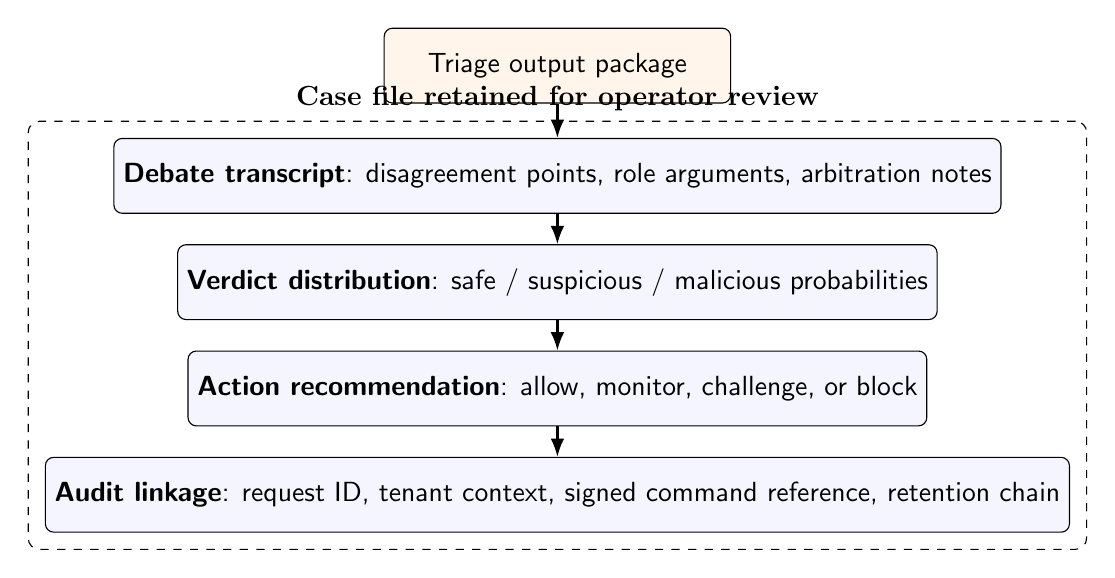
\begin{tikzpicture}[
  font=\sffamily,
  box/.style={draw, rounded corners=3pt, minimum width=8.2cm, minimum height=0.95cm, align=left, fill=blue!4},
  head/.style={draw, rounded corners=3pt, minimum width=4.4cm, minimum height=0.95cm, align=center, fill=orange!8},
  arrow/.style={-Latex, thick}
]

\node[head] (triage) at (4.1,5.2) {Triage output package};
\node[box] (transcript) at (4.1,3.8) {\textbf{Debate transcript}: disagreement points, role arguments, arbitration notes};
\node[box] (verdict) at (4.1,2.45) {\textbf{Verdict distribution}: safe / suspicious / malicious probabilities};
\node[box] (action) at (4.1,1.1) {\textbf{Action recommendation}: allow, monitor, challenge, or block};
\node[box] (audit) at (4.1,-0.25) {\textbf{Audit linkage}: request ID, tenant context, signed command reference, retention chain};

\draw[arrow] (triage) -- (transcript);
\draw[arrow] (transcript) -- (verdict);
\draw[arrow] (verdict) -- (action);
\draw[arrow] (action) -- (audit);

\node[draw, dashed, rounded corners=4pt, fit=(transcript)(verdict)(action)(audit), inner sep=6pt, label={[font=\bfseries]north:Case file retained for operator review}] {};

\end{tikzpicture}
\end{document}
